\documentclass[a4paper,12pt,titlepage]{article}

\usepackage{ucs}
\usepackage[T1]{fontenc}
\usepackage[utf8]{inputenc}
\usepackage[magyar]{babel}
\usepackage{amsfonts}
\usepackage{amsmath}
\usepackage{amssymb}
\usepackage{graphicx}
\usepackage[hang]{caption}
\usepackage{subcaption}
%\usepackage{enumerate}
%\usepackage{psfrag}
\usepackage[left=20mm,right=20mm,top=20mm,bottom=25mm]{geometry}
%\usepackage[left=10mm,right=10mm,top=10mm,bottom=15mm]{geometry} %landscape
\usepackage[hyphenbreaks]{breakurl}
\usepackage[hyphens]{url}
%\usepackage{multirow}
%\usepackage{booktabs}
\usepackage{hyperref}
%\usepackage{listings}
%\usepackage{csquotes}
\usepackage[range-phrase=--, range-units=single]{siunitx}
\usepackage{xcolor}
%\usepackage[a-3u]{pdfx}

\hypersetup{
	colorlinks,
	linkcolor={red!50!black},
	citecolor={blue!50!black},
	urlcolor={blue!80!black}
}

\pagestyle{plain} 

\listfiles % a package-ek kilistázása a logba

\title{
\centering

\includegraphics[width=0.6\textwidth]{kep/bme_logo.pdf} \\
\vspace{0.5cm}
\large{\textbf{Budapesti Műszaki és Gazdaságtudományi Egyetem}\\
\textbf{Villamosmérnöki és Informatikai Kar}\\
\textbf{Szélessávú Hírközlés és Villamosságtan Tanszék}}\\
\vspace{5cm}
\huge{\textbf{MSc Szakmai Gyakorlat Beszámoló}} \\
\vspace{3cm}}

%\parskip=10pt
%\parindent=0pt

\author{Szilágyi Gábor \\\vspace{2cm}\\ Konzulens: Bódi Tamás}
\date{Budapest, \today}
  

\begin{document}
    \maketitle
    \section{Bevezetés}
    A Silicon Laboratories Hungary kft-nél 2021 júliusában kezdtem el dolgozni gyakornokként és egészen 2022 augusztusáig maradtam a cégnél egy kisebb megszakítással télen. Az elmúlt évben sokat tanultam a munkám során. Az MSc-s szakmai gyakorlat ledokumentált időtartama alatt már komolyabb feladataim voltak, mint a gyakornokoskodásom elején. Ezeket az elvégzett feladatokat, a használt eszközöket és keretrendszert mutatom be ebben a beszámolóban. A cégen belül a ,,Hardware Tools'' csapatban dolgoztam, ez a csapat elsősorban a rádiós demonstrációs áramkörök tervezéséért és az ezekhez kapcsolódó mérésekért felelős.
    \subsection{A cégről}
        A fent említett cég a Silicon Laboratories (SiLabs) austini központú (USA, Texas), multinacionális vállalat budapesti alvállalata. A cég rendelkezik irodákkal Austinon és Budaesten kívül többek között Hyderabadban (India), Osloban (Norvégia) és Rennes-ben (Franciaország). A világ több sarkában való működés ellenére összesen körülbelül 2000-en dolgoznak a cégnél, a budapesti iroda jelenlegi létszáma 200 körüli, ami a cégen belül az egyik legnépesebb helyszínnek számít. Az egyes helyszínek valamelyest specializálódtak a feladatkörükben, például Austinban történik maguknak a szilícium chipeknek a fejlesztése, Budapesten hardver validációval és szoftverfejlesztéssel foglalkoznak nagy számban, norvégiában pedig a demonstrációs áramkörök gyártása történik.
        \par
        A SiLabs profilja a rádiós vagy rádió nélküli mikrokontroller integrált áramkörök (IC-k) tervezése, eladása, valamint hardveres és szoftveres támogatás nyújtása ezekhez az ügyfeleknek. Az ügyfelek nem végfelhasználók, hanem más cégek, akik a SiLabs chipjeit és támogatását felhasználva készítenek termékeket. Ilyen ügyfél például az Ikea, az Amazon, a Google és az Apple. Az Ikea példájánál maradva, a projekt, amivel személyesen találkoztam és ehhez az ügyfélhez köthető, az okos villanykörtékbe szánt rádiós modulok. Egy másik egyszerűbb alkalmazása a SiLabs rádióinak a kapunyitó távirányító, amikkel gyakran találkozom a laborban a munkatársaimnál. A komplexebb alkalmazások közé tartoznak az okos otthon kialakításához használható eszközök. Ilyen az Amazon Alexa nevű terméke, amely az okos otthon rendszer egy központi, irányító eleme lehet, de ennek a rendszernek más elemei is használhatnak SiLabs chipeket, mint például az okos szenzorok vagy vezérlőeszközök.
        \par
        A Hardware Tools csapat által tervezett és tesztelt demonstrációs áramkörök referencia implementációként szolgálnak a kérdéses IC-ket használó eszközökhöz. Ezeknek az áramköröknek a rádiófrekvenciás része főleg nagyobb frekvenciákon (pl. 2,4 GHz) nagyon érzékeny a nyomtatott áramköri rajz mintázatára és a beültetett alkatrészek elhelyezkedésére. Egy jól működő implementációtól való kis mértékű eltérés is nagyban ronthatja az áramkör teljesítőképességét több szempontból is. Ilyenkor legtöbbször az fordul elő, hogy az alapharmonikus frekvencián, ahol a hasznos adatátvitel történik, lecsökken a kisugárzott teljesítmény és a vételi érzékenység. Egy másik tünete a rosszul megtervezett NYÁK-nak a felharmonikus frekvenciákon a megnövekedett kisgugárzott teljesítmény. Az első probléma miatt az eszköz nem tudja elég jól vagy egyáltalán ellátni a feladatát, a második probléma miatt pedig más eszközök működését akadályozhatja, mivel nem felel meg az elelktromágneses kompatibilitási (EMC) követelményeknek.
        \par
        A csapat által tervezett demonstrációs kitek egy néhány évvel ezelőtti példánya látható \aref{fig:wstkmighty}. ábrán. A nagy Silicon Labs logóval ellátott alaplap a Wireless Starter Kit Mainboard, amit ,,WSTK'' néven szoktunk emlegetni. A kisebb, ,,Mighty Gecko'' feliratú NyÁK a ,,radio board'', amit a WSTK vezérel.
%
            \begin{figure}
                \centering
                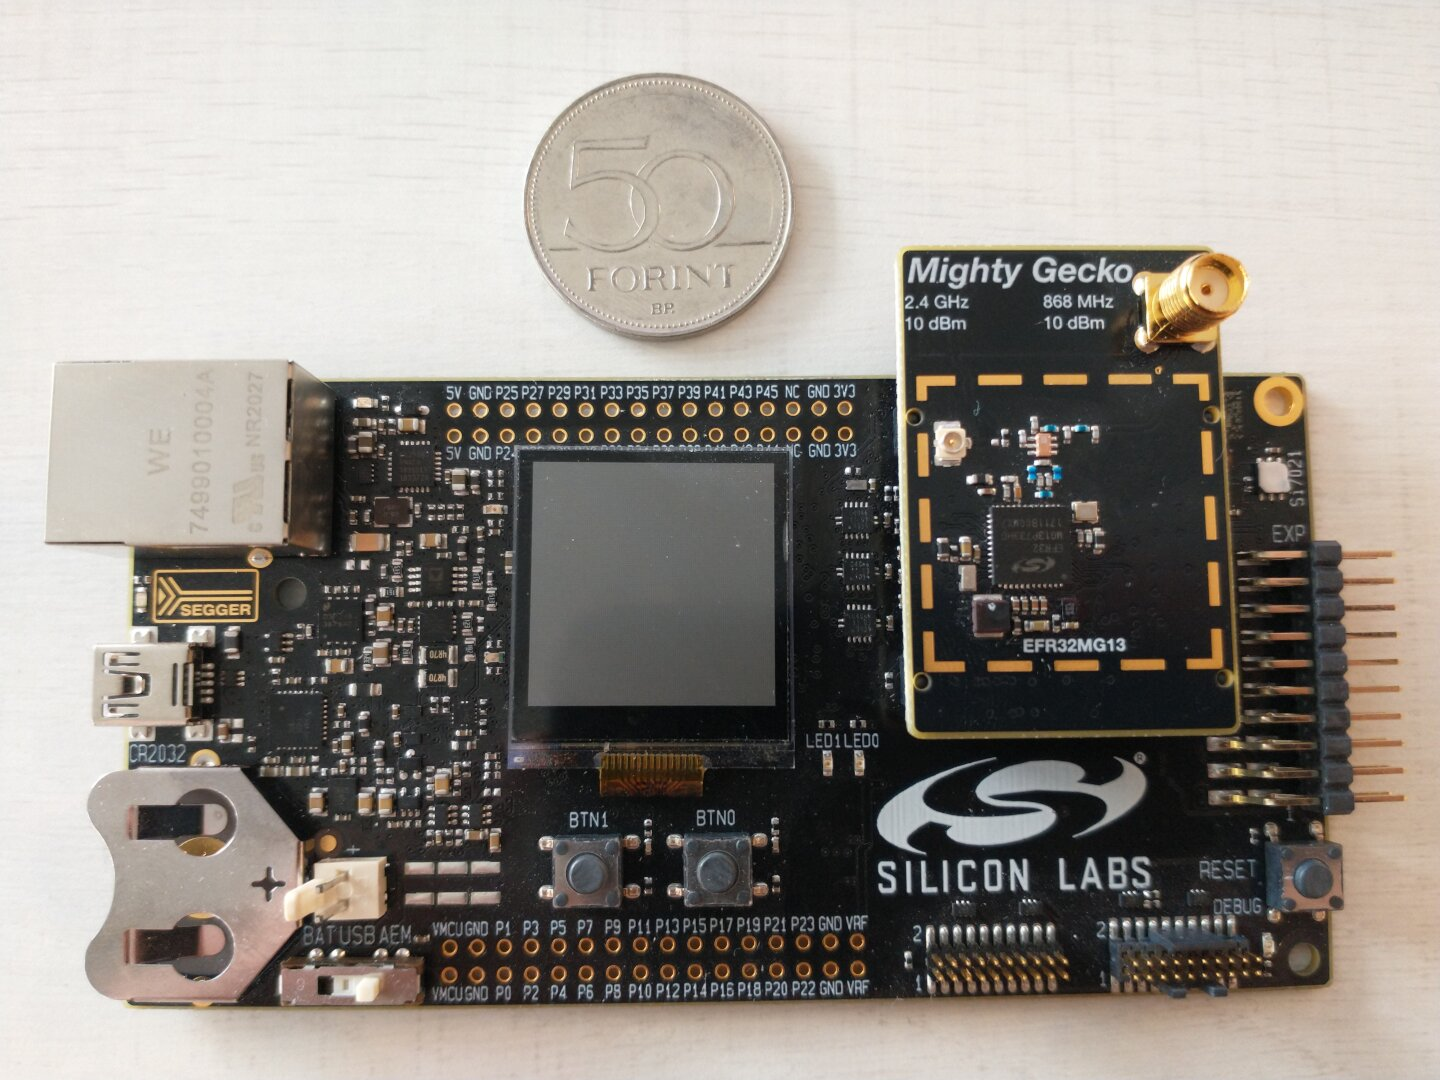
\includegraphics[width=0.8\textwidth]{kep/szerkesztett/wstk-mighty-gecko-nagy.jpg}
                \caption{WSTK + radio board.}
                \label{fig:wstkmighty}
            \end{figure}
%
    \section{Rádiófrekvenciás Mérés}
        A szakmai gaykorlatom során elsősorban a demonstrációs áramkörök rádiófrekvenciás részének fejlesztésével, tesztelésével foglalkoztam. A kérdéses áramköröknél rádiófrekvenciás (RF) szempontból a legtöbb fejfájást az antenna és a végfokerősítő közötti illesztőhálózat okozza. Ez a hálózat azokon az áramkörökön, amikkel én találkoztam, legtöbbször egy 5-elemű szűrő- és illesztőfokozat, ami diszkrét tekercsekből és kondenzátorokból van felépítve az NyHL-en. Egy másik alkatrész, amit elsősorban szub-\SI{}{GHz}-en használnak a cégnél, az integrált balun használata, ami \aref{fig:wstkmighty}. ábrán lehet kivehető az U.FL csatlakozótól jobbra a ,,Mighty Gecko'' feliratú NyHL-en, mint barna, hatlábú alkatrész. Az illesztőhálózatnak sokféle változata van használatban a különböző áramkörökön, mert több szempont határozza meg együttesen az ideális tulajdonságokat.
        \par
        Az első és legnyilvánvalóbb ilyen szempont a működési frekvencia. Értelemszerűen ha más frekvencián működik a rádió, akkor más elemértékekkel lehet hasonló szűrő és impedanciaillesztő hatást elérni. A gyakran előforduló működési frekvenciák: \SI{2,4}{GHz}, \SI{915}{MHz}, \SI{868}{MHz} és \SI{470}{MHz}, de előfordulhatnak még olyanok, amikkel csak én nem találkoztam a munkám során, de tervez ilyen frekvenciákra is eszközöket a cég. Ezek elsősorban \SI{915}{MHz} vagy \SI{470}{MHz} környékén lehetnek, amelyik tartományokban tudtommal a világ különböző részein más-más frekvenciasáv van kijelölve ISM (Industrial Scientific Medical) használatra, amilyen sávokban ezek az eszközök működhetnek. Az elemértékek meghatározásán kívül még egy érdekes hatása van a működési frekvenciának az áramkör tervezésénél. A \SI{2,4}{GHz}-es és szub-\SI{}{GHz}-es áramköröknél jelentős különbség van abban, hogy mennyire érzékeny az illesztőhálózat viselkedése a struktúra geometriájára. Nem meglepő módon nagyobb frekvencián, ahol a működési hullámhossz, de főleg a felharmonikus hullámhosszak közelebb vannak az RF áramköri rész méreteihez, a viselkedést komolyan befolyásolja a geometria. Ezzel szemben nagyobb hullámhosszaknál ez a hatás lecsökken és sokkal szabadabban lehet átrendezgetni az NyHL-en az alkatrészeket mindenféle helytakarékossági és egyéb szempont alapján, persze a topológia megtartásával.
        \par
        Egy másik szempont az illesztőhálózat tervezésénél a rádió végfokerősítőjének a kimeneti impedanciája. Az illesztőhálózat egyik fontos feladata, hogy kis reflexióval és veszteséggel illessze a végfok kimeneti impedanciáját a NyHL-en található \SI{50}{OHm}-os mikroszalagvonalhoz (microstrip line). Az egyes rádiós IC-k többféle teljesítményszinttel készülnek, így még egy típuson belül is többféle végfokerősítőhöz kell különböző illesztőhálózatot tervezni. A gyakran előforduló teljesítményszintek közül néhány: \SI{0}{dBm}, \SI{6}{dBm}, \SI{10}{dBm}, \SI{14}{dBm}, \SI{16}{dBm} és \SI{20}{dBm}.
        \par
        Még egy fontos szempontcsoportot alkotnak a hordozó paraméterei. Ilyenek például a szubsztrát dielektromos állandója és a rézrétegek közötti távolság. Mindkettő a parazita hatások kialakulásában játszik fontos szerepet, emiatt előfordul, hogy csak a rézrétegek közötti hézag változtatása miatt (pl. áttérés 4 rétegű hordozóról 2 rétegűre) teljesen újra kell tervezni az illesztőhálózatot. A fenti példában a nagyobb rétegtávolság a szomszédos rézrétegek között csökkenti a parazita kapacitást, ugyanakkor megnöveli a szomszédos rétegek között kialakuló áramhurok hosszát, így növelve annak az áramútnak parazita induktivitását. Hasonló jelenségek miatt ilyen helyzetben könnyen lehet, hogy még az illesztőhálózat topológiáján vagy elemszámán is változtatni kell, hogy megfelelően működjön.
        \subsection{Vezetett mérés}
            Az általam rendszeresen végzett RF mérések közül a vezetett mérés az egyszerűbb. Ez gyakorlatilag abban áll, hogy a radio board RF kimenetét, ami egy U.FL vagy SMA csatlakozó, egy spektrumanalizátorra kapcsolom és a kiadott jelet elemzem. Ilyen méréseknél általában egy egyszerű szinuszos jelet generáltatok a radio boarddal és az alapharmonikus, valamint a felharmonikusok teljesítményszintjeit vizsgálom. Ilyen célra legtöbbször az Anritsu MS2692A típusú spektrumanalizátort használtam, ami \aref{fig:anritsu}. ábrán látható, mert ennek a műszernek elég alacsony a zajszintje. Két ilyen mérési eredmény látható \aref{fig:sol-conducted}. ábrán, ahol megfigyelhető, hogy a más frekvenciára készült két testvér radio board közül (mindkettő rádiós chipje a ,,Sol'' cégen belül használt kódnév alatt) a \SI{470}{MHz}-esnek kisebbek a felharmonikus teljesítményei. Tudtommal alacsonyabb frekvencián szigorúbbak a követelmények a felharmonikus teljesítményekkel szemben, mégis az a tapasztalat, hogy alacsonyabb frekvenciájú board-okon kisebb problémát okoznak a felharmonikusok, nagyobb szokott lenni a tartalék a ténylegesen kimért teljesítményszintek és az EMC szabványban meghatározottak között.
            \par
%
            \begin{figure}
                \centering
                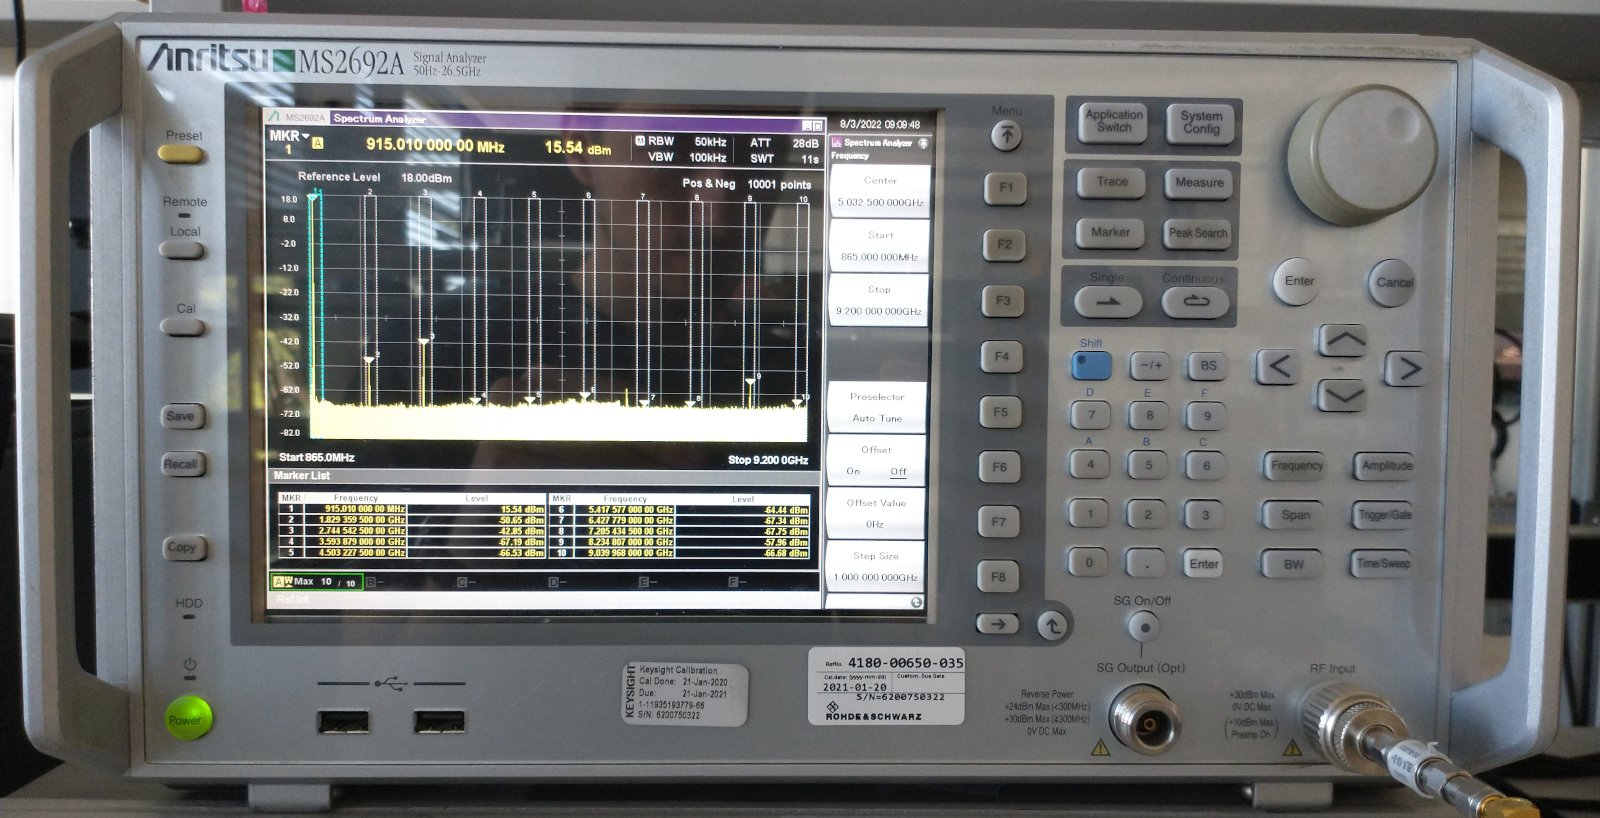
\includegraphics[width=0.6\textwidth]{kep/szerkesztett/anritsu.jpg}
                \caption{Anritsu MS2692A}
                \label{fig:anritsu}
            \end{figure}
%
            Vezetett mérést elsősorban két helyzetben végeztem. Egyrészt skkor, amikor már egy más téren letesztelt radio boardról el kellett dönteni, hogy megfelel-e a szabványnak a vezetett teljesítményszintek alapján. Ugyan rádiókról van szó, így elvileg elég lehetne kizárólag csak a sugárzott teljesítményszinteket vizsgálni, de szükség van a vezetetten kicsatolt kimeneti jel minőségbiztosítására is, hogy megfeleljen a szabványnak. A második helyzet, amikor vezetett méréseket végeztem, az volt, amikor egy radio board diszkrét alkatrészekből kialakított illesztőhálózatát kellett próbálkozás útján tökéletesíteni, majd minden változtatás után dokumentálni az adódó teljesítményspektrumot. A \SI{2.4}{GHz}-nél fellépő jelentős parazitahatások miatt gyakorlatilag lehetetlen lenne jó áramköri modellt alkotni a kérdéses illesztőhálózathoz, a 3D-s elektromágneses szimuláció előkészítése pedig túl hosszadalmas lenne, így maradt a próbálkozásos és méregetős módszer. Szub-\SI{}{GHz}-en nem okoztak ilyen gondot az illesztőhálózatok, ilyen board-okon elegendő volt a régen kikísérletezett, jól bevált illesztőhálózatok használata, főleg, hogy amint fentebb említettem, szub-\SI{}{GHz}-en szabadabban lehet a geometriát változtatni, így sokféle elrendezésnél használható marad a megegyező topológiájú hálózat.
            \begin{figure}
                \centering
                \begin{subfigure}{0.48\textwidth}
                    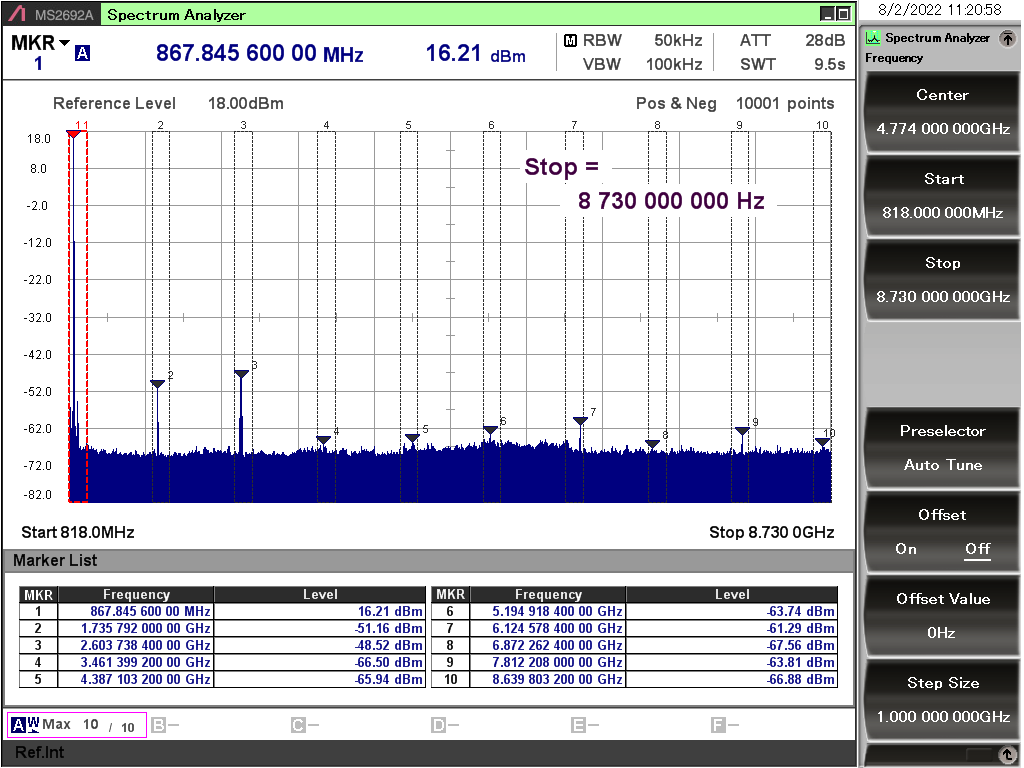
\includegraphics[width=\textwidth]{kep/szerkesztett/sol-868-conducted.png}
                    \caption{\SI{868}{MHz}}
                \end{subfigure}
                \begin{subfigure}{0.48\textwidth}
                    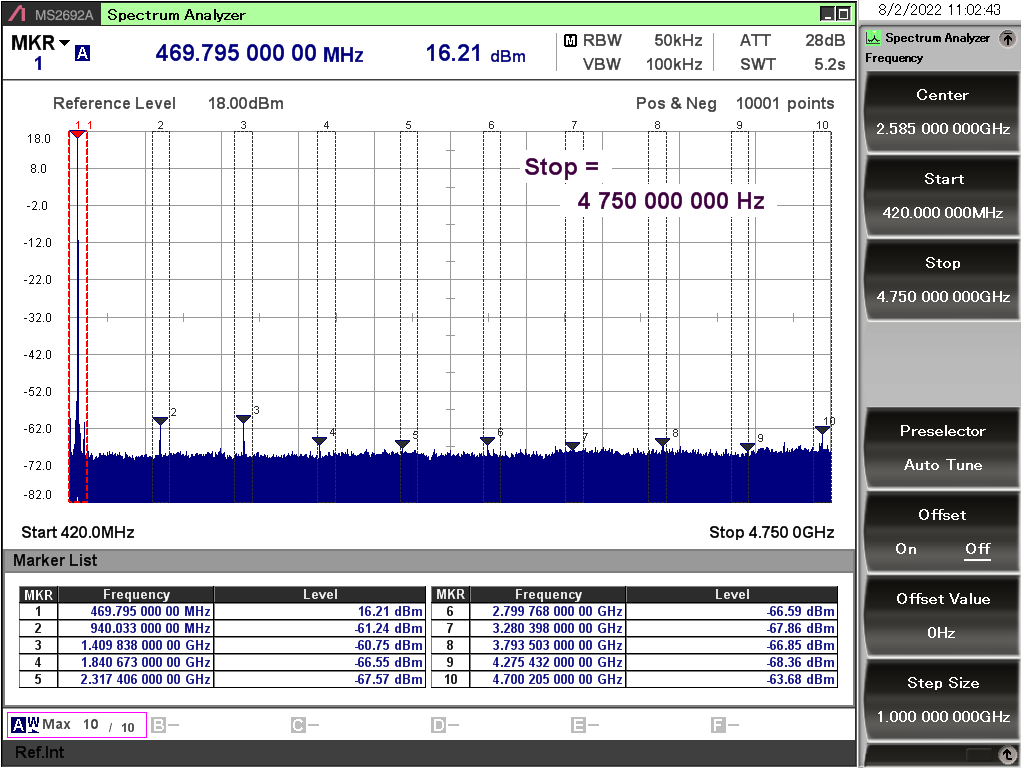
\includegraphics[width=\textwidth]{kep/szerkesztett/sol-470-conducted.png}
                    \caption{\SI{470}{MHz}}
                \end{subfigure}
                \caption{470 és \SI{868}{MHz}-es Sol radio board-ok kimeneti spektruma.}
                \label{fig:sol-conducted}
            \end{figure}
%
        \subsection{Sugárzott mérés}
            A vezetett mérés mellett a másik módszer, ahogy egy radio board teljesítőképességét vizsgáltuk a sugárzott mérés, amihez a budapesti irodában lévő antennaszobát használtuk. Maga az antennaszoba egy RF szempontból külső zajoktól elszigetelt és belül a felületeket borító tüskékkel reflexiócsökkentett helyiség. Bent található egy mérőantenna, kicsit pontosabban egy bordás tölcsérantenna, aminek ismert a nyereség-frekvencia karakterisztikája körülbelül \SI{0,3}{GHz}-től \SI{15}{GHz}-ig. Az antennától \SI{3}{m}-re található egy hungarocelltorony léptetőmotorral az alján, ami forgóasztalként funkcionál. Erre az asztalra tesszük méréshez a vizsgálandó rádióadót, vagyis a DUT-ot (Device Under Test) és az antennára csatlakoztatott spektrumanalizátor segítségével mérjük a különböző irányokban és frekvenciákon kisugárzott teljesítményt. Az antennaszoba két vége \aref{fig:antennaszoba}. ábrán látható.
            \begin{figure}
                \centering
                \begin{subfigure}{0.4\textwidth}
                    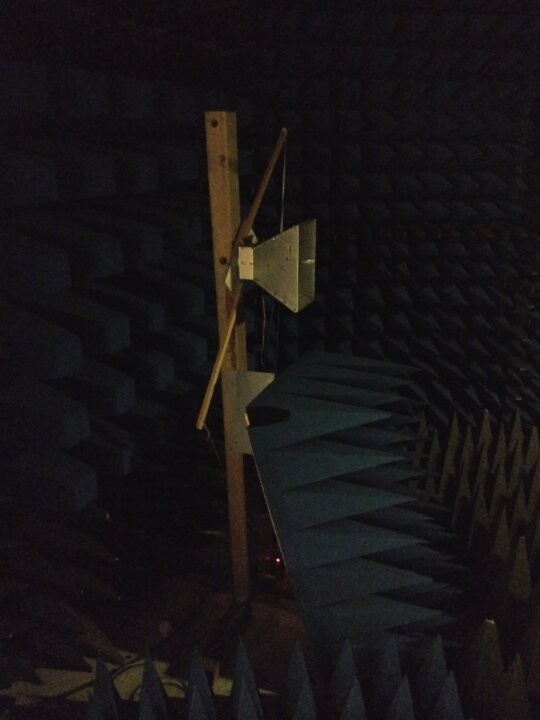
\includegraphics[width=\textwidth]{kep/szerkesztett/antennaszoba-antenna.jpg}
                    \caption{Mérőantenna}
                \end{subfigure}
                \begin{subfigure}{0.4\textwidth}
                    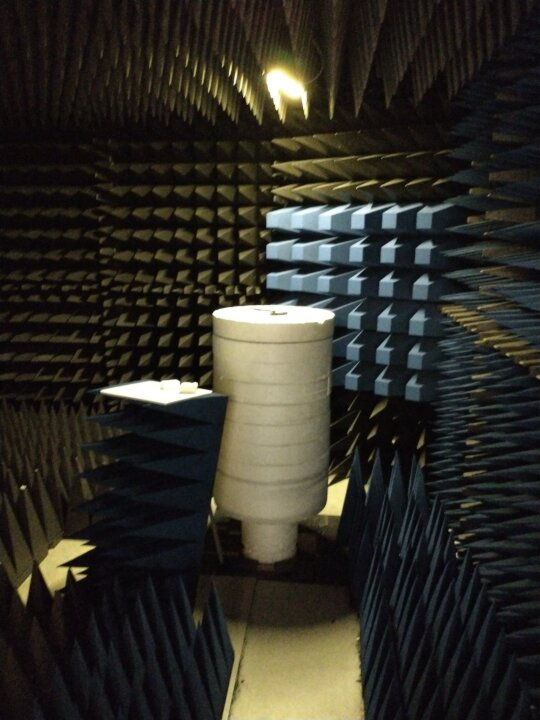
\includegraphics[width=\textwidth]{kep/szerkesztett/antennaszoba-asztal.jpg}
                    \caption{Forgóasztal}
                \end{subfigure}
                \caption{Berendezés az antennaszobában.}
                \label{fig:antennaszoba}
            \end{figure}
            \par
            Az antennaszobának van egy előszobája, ami már a leárnyékolt helyiségen kívül van, itt található a sugárzott mérésekhez dedikált Rohde \& Schwarz FSQ típusú spektrumanalizátor, a szobában található léptetőmotorok vezérlője és az egész mérést irányító számítógép, ami az előszoba többi eszközére van csatlakoztatva. Az antennaszobában háromféle mérést lehet végezni, ezek közül én kettővel foglalkoztam, de a harmadik mérés tárgyához, egy speciális radio boardhoz is volt valamennyi közöm.
            \par
            Az első méréstípus a harmonikus teljesítményszint mérés, röviden ,,performance'' mérésként szoktuk emlegetni. Ebben az esetben a tesztelni kívánt adót a forgóasztalra helyezzük és az egy helyben álló mérőantenna segítségével mérjük az antennához érkező teljesítmény maximumát, amíg körbefordul az asztal a DUT-tal. Ezáltal a DUT 3-dimenziós iránykarakterisztikájának egy bizonyos síkmetszetén belül tudjuk meghatározni a maximális kisugárzott teljesítménysűrűséget. A DUT-ot a forgóasztalra \aref{fig:orientaciok}. ábra szerinti orientációkban helyezhetjük el.
%
            \begin{figure}
                \centering
                \begin{subfigure}{0.3\textwidth}
                    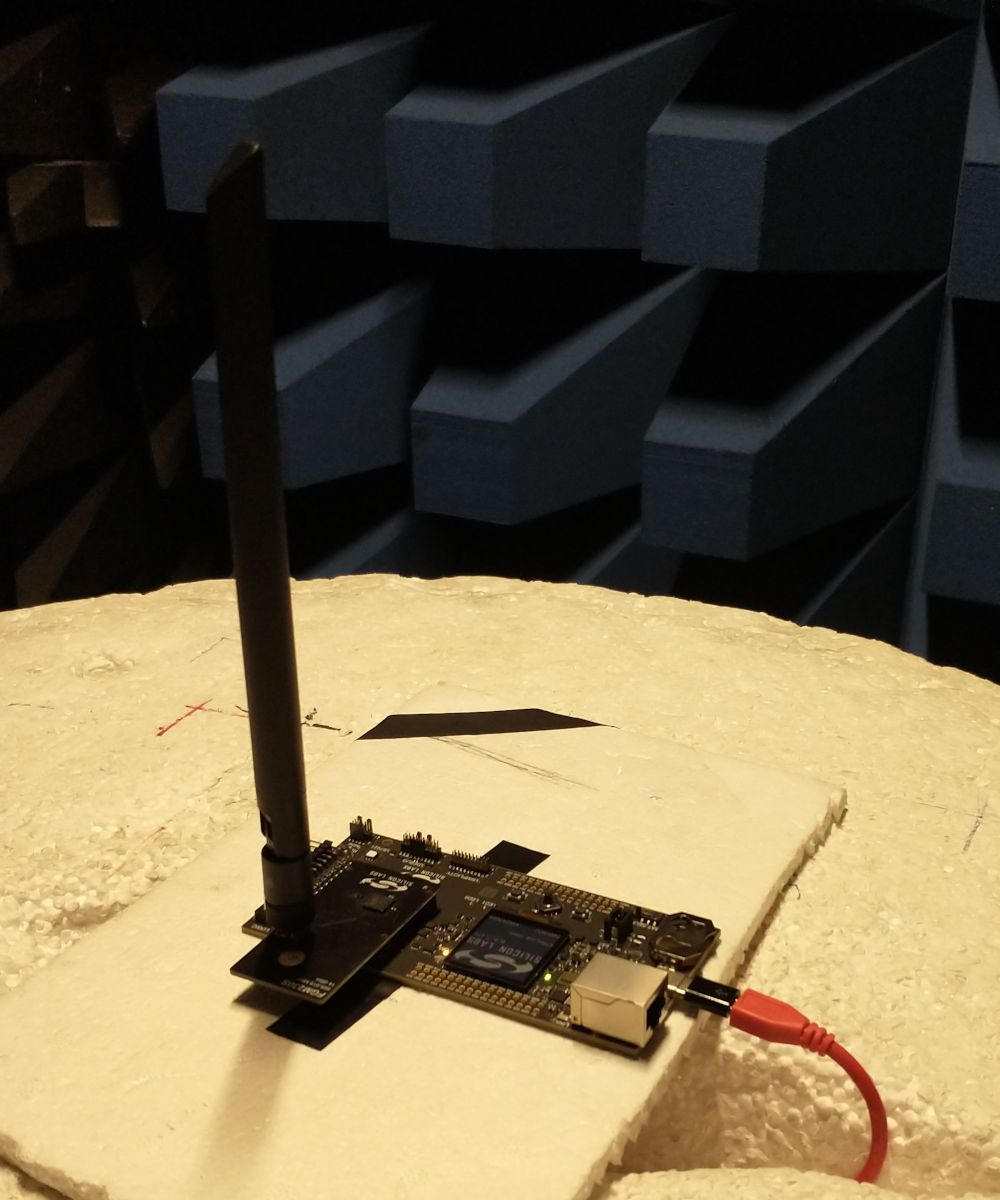
\includegraphics[width=\textwidth]{kep/szerkesztett/botantenna_XY.jpg}
                    \caption{XY sík}
                \end{subfigure}
                \begin{subfigure}{0.3\textwidth}
                    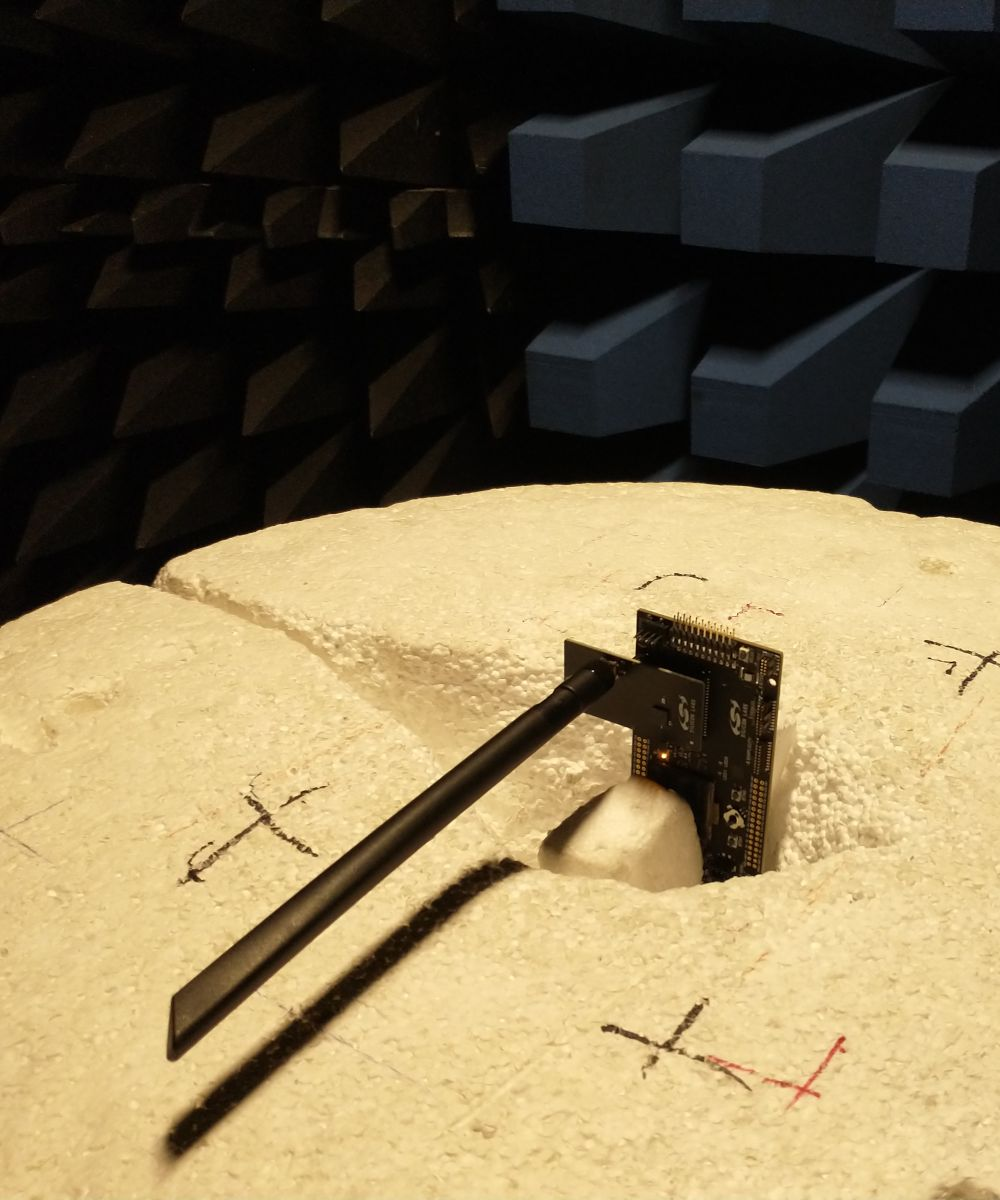
\includegraphics[width=\textwidth]{kep/szerkesztett/botantenna_XZ.jpg}
                    \caption{XZ sík}
                \end{subfigure}
                \begin{subfigure}{0.3\textwidth}
                    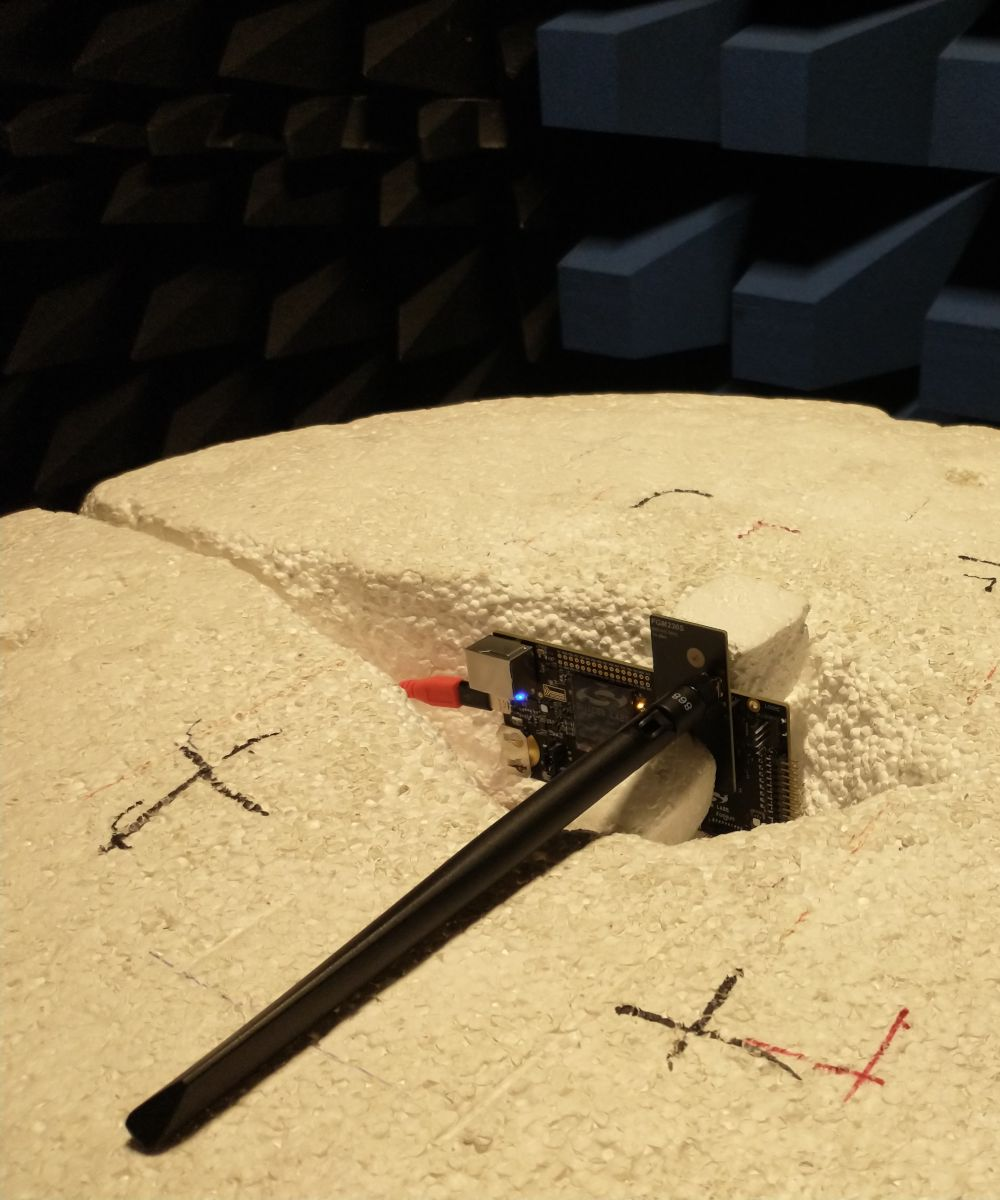
\includegraphics[width=\textwidth]{kep/szerkesztett/botantenna_YZ.jpg}
                    \caption{YZ sík}
                \end{subfigure}
                \caption{Az iránykarakterisztika három metszetének mérése az antennaszobában.}
                \label{fig:orientaciok}
            \end{figure}
%
            A performance méréshez hozzátartozik még az, hogy milyen frekvencián mérünk, pontosabban az alapharmonikus hányadik felharmonikusán (vagy magán az alapharmonikuson). Ez gyakorlatilag csak a spektrumanalizátor vezérlésének és a mért nyers teljesítményszintek korrekciójának kérdése. Még egy fontos mérési paraméter a mérőantenna polarizációja, ami szerint vízszintes és függőleges orientációjú méréseket szoktunk végezni. Összességében a performance mérésnél tehát a paraméterek: az alapharmonikus frekvencia, a felharmonikus sorszáma, a DUT orientációja és a mérőantenna polarizációja. A performance méréseknél általában az a lényeges adat, hogy minden mért orientációban, polarizációval és felharmonikuson megfelel-e az EMC követelményeknek a DUT. Ha a mérés alapján megfelel, akkor elég jó biztossággal lehet állítani, hogy a le nem tapogatott irányokban nincs kiugró nyaláb a felharmonikusok sugárzásában, tehát tényleg megfelel a követelményeknek. Ha esetleg nem ment át a teszten, akkor a mérés paramétereiből lehet valamelyest arra következtetni, hogy honnan jöhet a nemkívánt felharmonikus sugárzás, esetleg mivel lehetne ezt orvosolni.
            \par
            Egy másik antennaszobai mérés az iránykarakterisztika mérése. A mérés előkészítése fizikailag ugyanabból áll, mint a performance mérés esetében. Annyi a különbség, hogy itt csak az alapharmonikuson szoktunk mérni (a felharmonikusok sugárzásának karakterisztikája érdektelen, ha a megadott küszöbszint alatt vannak), valamint amért teljesítményszintek feldolgozásában. A spektrumanalizátor zero span módban az alpharmonikus frekvencián mér, amíg a forgóasztal egyszer körbefordul a DUT-tal, addig ezzel szinkronban a spektrumanalizátor egyet sweepel, így a körbefordulás végére a kijelzőjén megjelenik az adott síkhoz tartozó iránydiagram derékszögű koordinátarendszerben ábrázolva.
        \subsection{Modulációs faktor}
            Az EMC szabványok szerint a valós alkalmazás körülményei között kell az eszköznek megfelelnie a felharmonikusok teljesítményszintjeivel szemben támasztott követelményeknek. A laborban a méréseket viszont CW (Continous Wave), vagyis modulálatlan vivő adása mellett teszteljük. Azért van erre szükség, mert modulált jelnél a felharmonikus frekvenciák körül szétkenődött jel spektrális teljesítménysűrűsége olyan kicsi, hogy a zajszint alá kerül, emiatt nem lehet effektíven megmérni. Megjegyzem, hogy gyakorlatilag a CW jel modulációja nem hat a kimeneti jel összteljesítményére, tehát a moduláció az adott, CW esetben egyszerűen mérhető jelteljesítményt nem növeli vagy csökkenti, csak nagyobb sávszélességen osztja el. A boardjainkat érintő szabvány kiköti, hogy a megfelelőség eldöntéséhez használt spektrumanalizátoron \SI{1}{MHz}-es RBW (Resolution BandWidth) legyen beállítva, ami egyszerre csak közelítőleg egy \SI{1}{MHz} széles frekvenciasávba eső összteljesítmény mérését jelenti. A modulálatlan jel sávszélessége nagyon kicsi, habár nem 0, mivel elég kicsi a rádió oszcillátorának fáziszaja. Egy konzervatív felső becslésként vegyük ezt a sávszélességet \SI{1}{kHz}-nek, a konkrét jellemző értékekre nem emlékszem. Az alapharmonikuson ülő jelkomponens sávszélességének $n$-szerese az $n$-edik felharmonikus körül ülő komponens sávszélessége. Eszerint még a sokadik felharmonikus frekvencia körül is csak nagyon kis sávszélességet foglalna el a jel, például a 20. harmonikus körül is csak \SI{\pm10}{kHz}-et, ami még bőven teljesen bele esik a megadott \SI{1}{MHz}-es sávba. Ha a fentiekkel szemben nem CW jellel mérünk, hanem valamilyen szélesebb frekvencialöketű modulált jellel, akkor könnyen elképzelhető, hogy már a 3--4. harmonikus frekvencia környékén is a keltett zavaró jelkomponens sávszélessége lényegesen szélesebb, akár többszörösen is, mint az emlegetett \SI{1}{MHz}-es határ. Emiatt akármelyik konkrét frekvencia környezetében végezzük is a mérést, a mérésnél használt RBW-t meghatározó szűrő az adott harmonikus környékén szétszórt jelteljesítménynek mindig csak egy részét engedi át, ez pedig csökkenti a modulált mérésnél kapott harmonikus teljesítményszinteket a CW mérés eredményeihez képest. A két mérési eredmény eltérése a modulációs faktor (lineáris skálán a két összetartozó teljesítményszint hányadosa; logaritmikus skálán, például \SI{}{dBm}-ben megadott teljesítmények számértékének különbsége \SI{}{dB}-ben).
            \par
            Ez alapvetően egy előnyös dolog, de azért hogy teljesen kihasználhassuk a jelenségben rejlő lehetőségeket, kicsit mérni és számolni kell. A fentiek miatt a CW (modulálatlan) jellel végzett mérés a lehető legszigorúbb a moduláció szempontjából. Tehát ha egy rádió CW esetben átmegy a teszten, akkor biztosak lehetünk benne, hogy modulált esetben is átmenne, mert az eredmény nem lehetne rosszabb, legfeljebb hasonló, kislöketű modulációk esetén. Akkor lesz érdemes a modulációs faktoral számolni, ha a rádió megbukik a teszten, de nem sokkal, például csak 2--3 {}{dB}-vel. Ekkor egyszerűen a modulációs faktort ki kell vonni a mért teljesítményszintből és az így kapott, kompenzált értéket kell összehasonlítani a szabványban megadott határértékkel. Mint fent említettem, az aktuális modulációs faktor függ a felharmonikus sorszámától és a modulációs eljárástól. A Silabs-féle rádiós IC-k többféle modulációt támogatnak, az egyes modulációs eljárásokon belül (BPSK, QAM, stb.) is többféle változat használható, más-más bitsebességgel és frekvencialökettel, ezáltal sávszélességgel.
            \par
            Az egyes lényeges modulációkra érdemes megmérni a modulációs faktort lehetőleg olyan műszerbeállításokkal, amilyenekkel a hivatalos EMC teszteket is végeznék. Ez volt az én egyik feladatom. A méréseket \aref{fig:fsv}. ábrán látható spektrumanalizátorral végeztem. Ennek a műszernek ugyan nincs kvázicsúcs-detektora, amilyen csak nagyon drága műszerekben szokott előfordulni és a hivatalos teszteken is használatos, de ilyen téren is lehet a szigorúbb döntés felé hibázni. Ez a szigorúbb mérést eredményező detektor a csúcsdetektor, emiatt ilyet használtam a méréseken.
 %
            \begin{figure}
                \centering
                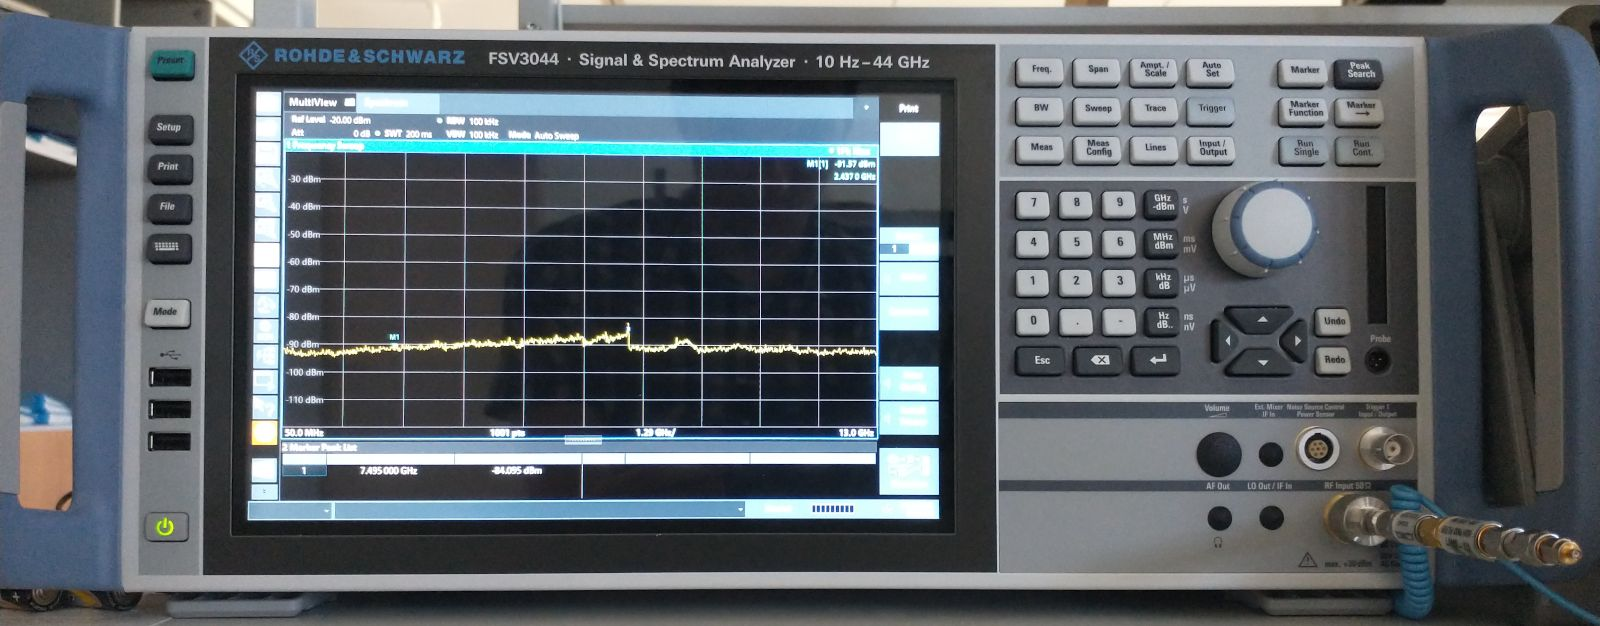
\includegraphics[width=0.6\textwidth]{kep/szerkesztett/fsv.jpg}
                \caption{Rohde \& Schwarz FSVA3044 Spektrumanalizátor.}
                \label{fig:fsv}
            \end{figure}
%
   \section{NyHL tervezés}
        A cég által forgalmazott rádiós IC-ket használó referencia-áramkörök, leginkább az ezeket hordozó nyomtatott huzalozási lemezek tervezése a Hardware Tools csapat feladata, így ebben is részt vettem. Az egyik folyó projekt egy olyan készülékpáros tervezése volt a cégnél, ami rádiós komunikáció alapján képes nagy pontossággal távolságo mérni két kisméretű résztvevő eszköz között. A projektet ,,HADM'' (vagyis ,,High Accuracy Distance Metering'') néven emlegettük. A két résztvevő készülék nem egyforma, az egyik egy egyszerű adóvevő, ez a ,,tag'', ami körülbelül akkora, mint egy kézi rádiós kaputávirányító, a másik pedig egy komolyabb, többantennás mérőműszer. Az utóbbi végeredményben jelzést küld a tag-nek, ami válaszol, majd a válaszjel érkezési ideje és egyéb paraméterei alapján lehet kiszámítani a távolságot a két készülék között.
        \par
        A HADM projektbe annyival segítettem be, hogy a tag layoutjának megtervezésébe segítettem be. Ehhez az Altium Designer szoftvercsomagot használtam, amit a cégnél, de elsősorban a Hardware Tools csapatban előszeretettel használnak. Az Altium Designer az NyHL tervezés minden lépését magába foglalja erősen integrált módon, a kapcsolási rajz tervezésétől a layout megszerkesztésén át a gyártási fájlok generálásáig. Ilyen szempontból hasonlít a KiCAD-hez, ami gyakorlatilag egy ingyenes és nyílt forráskódú megfelelője az Altium Designer-nek, persze sok funkció hiányzik belőle, amit az Altium Designer nyújt, lévén az utóbbi egy meglehetősen borsos árú, professzionális programcsomag. Azzal, hogy előzőleg már saját szórakozásomra terveztem NyHL-t KiCAD-ben és a cégnél egy professzionálisabb program használatával is kipróbálhattam magam
        \subsection{Kapcsolási rajz}
        \subsection{Nyomtatott huzalozási rajz}
            \begin{figure}
                \centering
                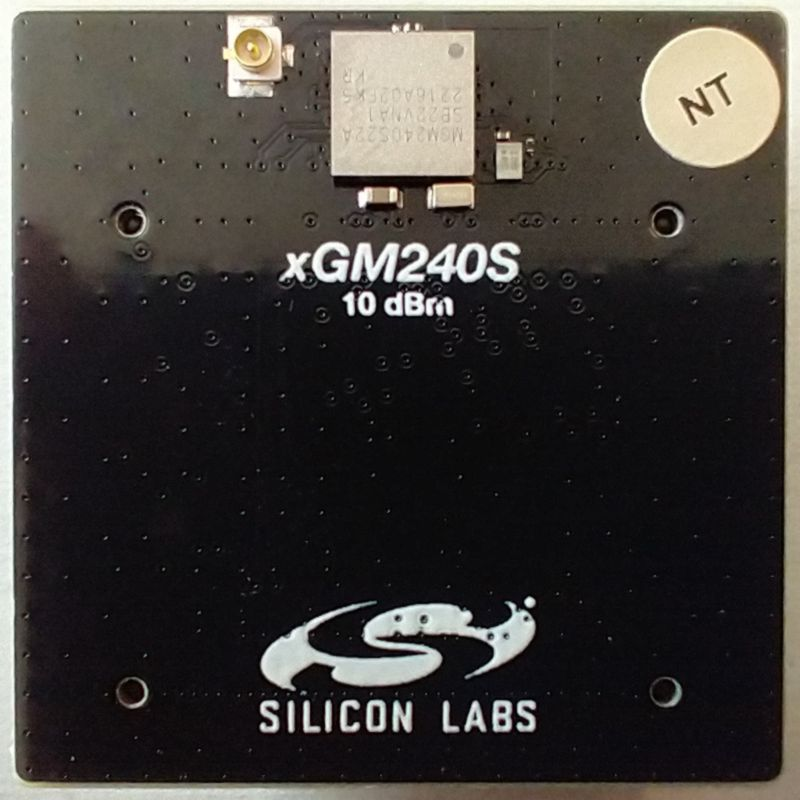
\includegraphics[width=0.6\textwidth]{kep/szerkesztett/sip-modul.jpg}
                \caption{sip-modul}
                \label{fig:sip}
            \end{figure}
%
            \begin{figure}
                \centering
                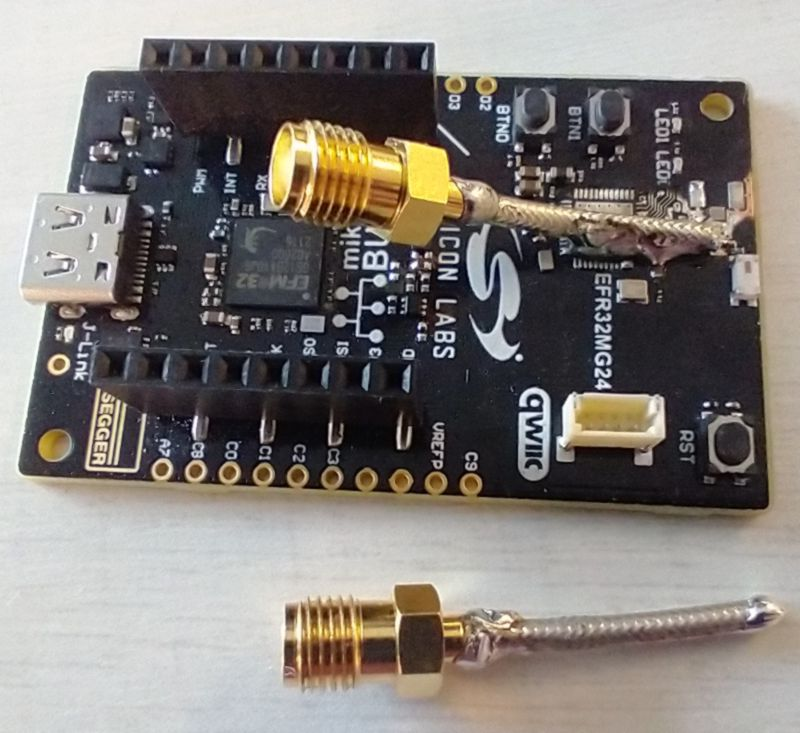
\includegraphics[width=0.48\textwidth]{kep/szerkesztett/pigtail1.jpg}
                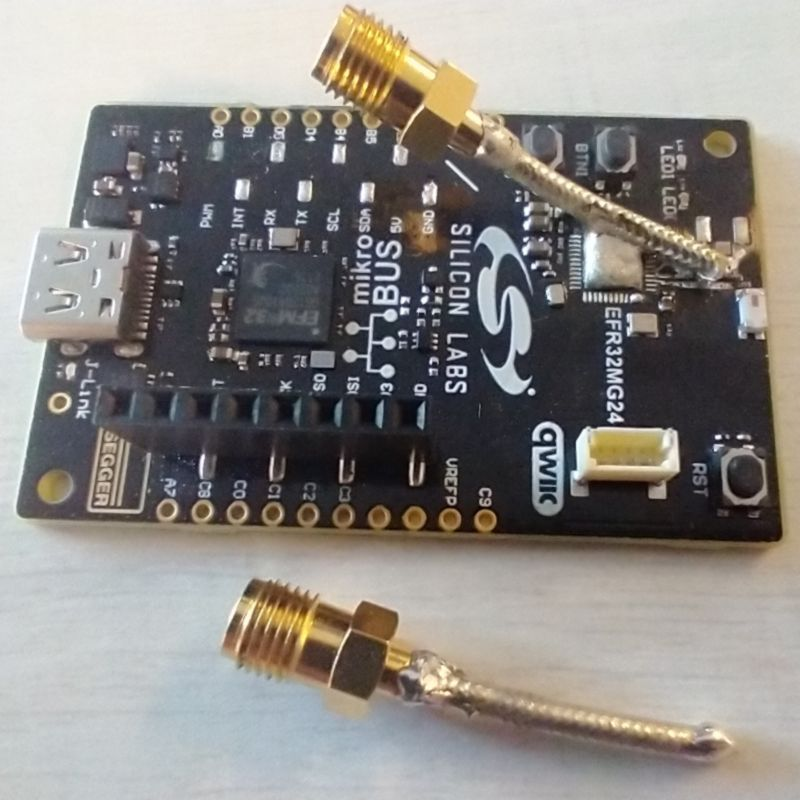
\includegraphics[width=0.48\textwidth]{kep/szerkesztett/pigtail2.jpg}
                \caption{pigtailek}
                \label{fig:pigtail}
            \end{figure}
%
            \begin{figure}
                \centering
                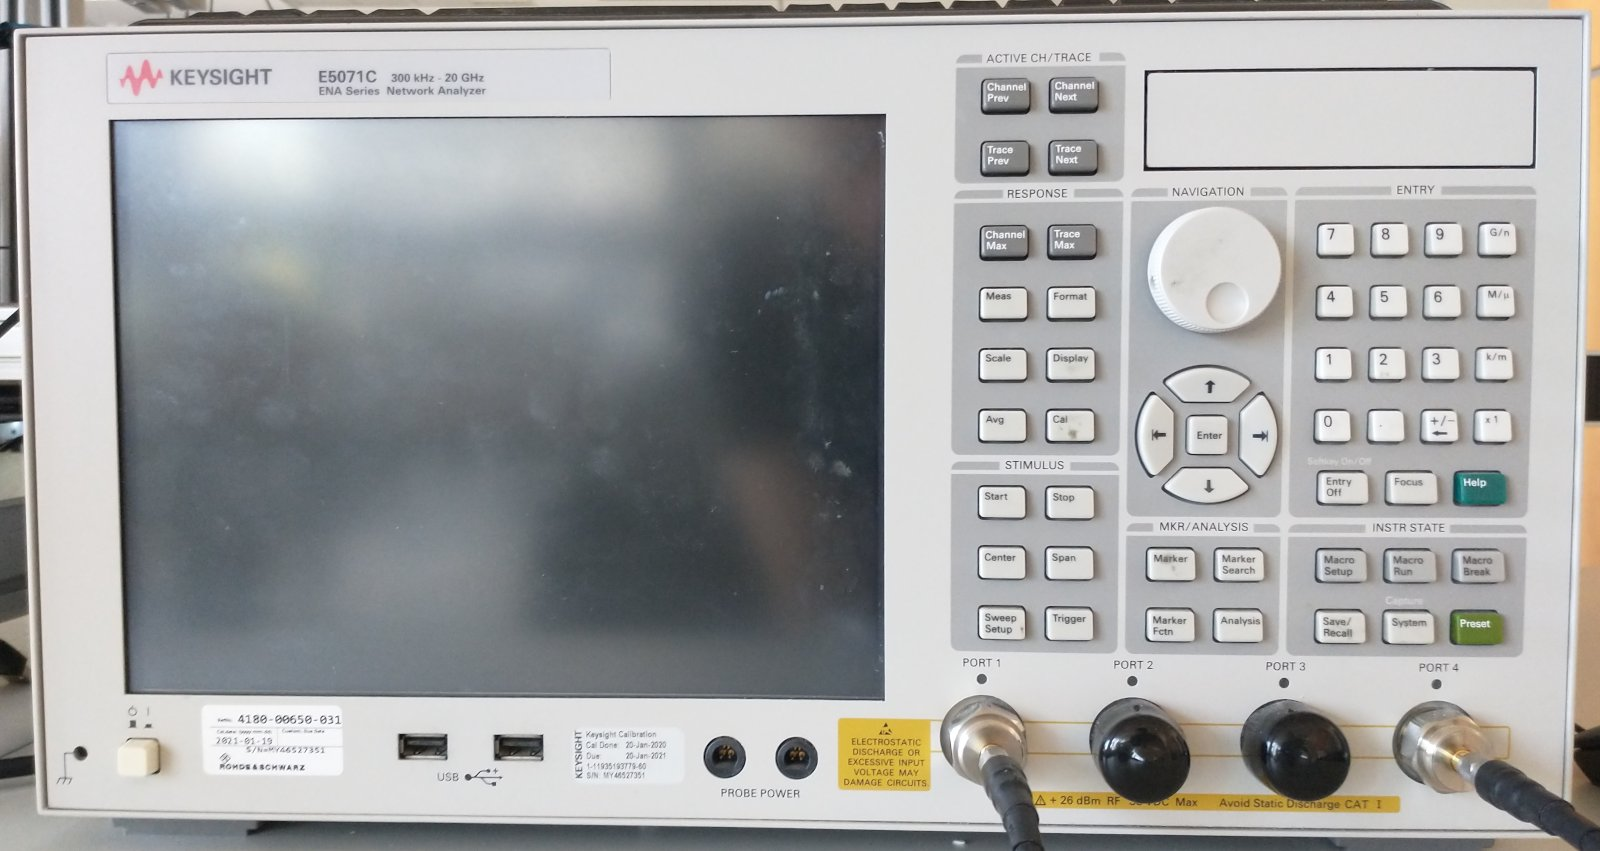
\includegraphics[width=0.6\textwidth]{kep/szerkesztett/vna.jpg}
                \caption{VNA}
                \label{fig:vna}
            \end{figure}
%
%
            \begin{figure}
                \centering
                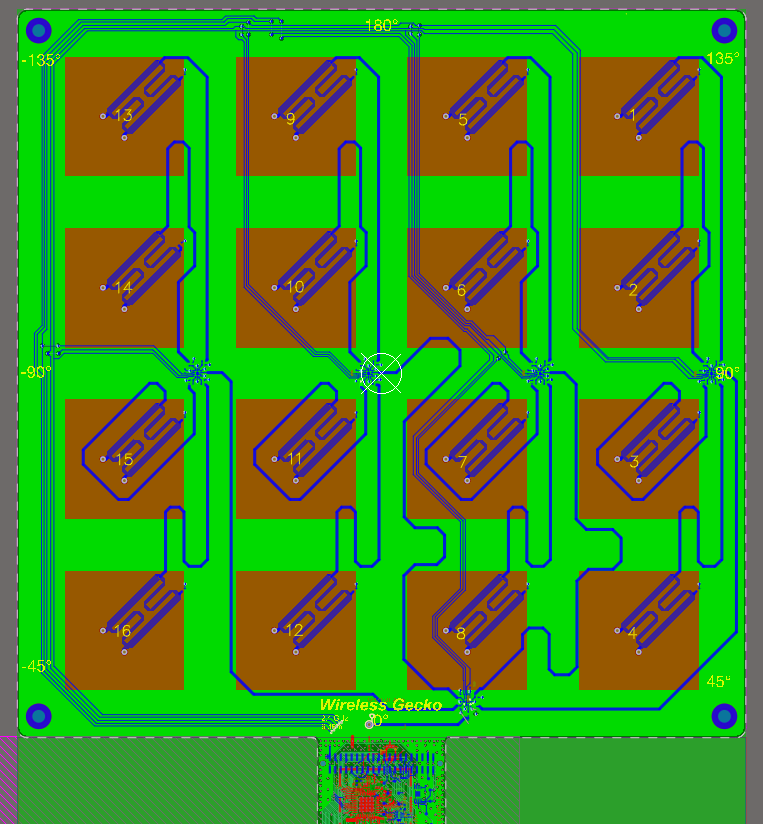
\includegraphics[width=0.6\textwidth]{kep/szerkesztett/antennamatrix.png}
                \caption{Beltéri iránymérő antennamátrix.}
                \label{fig:antennamatrix}
            \end{figure}
%
\end{document}
